\section{How it works}
\label{sec:qr_functioning}

Graphically, QR-Codes are composed of black and white squares called "modules". Each module represents a binary bit, black meaning 1, white meaning 0.

Similarly to \autoref{sec:barcode_functioning}, we will only describe the encoding phase.

To make the following explanations easier to follow, we will use a concrete value.

Let's encode the string "Hello, World!" with level "M" of error correction.

\subsection{Data type}
\label{ssec:qr_data_type}

The first step is to choose the appropriate data type for encoding. In our case, we can't use the numerical format since there are letters, nor can we use the alphanumerical, because of the exclamation mark and lowercase letters. Thus, the most suitable encoding is the byte format.

Note that these different formats exist to optimize encoding to take the least possible space, so it is recommended to choose the minimum required format to avoid unecessarily big QR-Codes.

The first 4 bits of data in our code will be the format used. Numerical is 1, alphanumerical is 2, byte is 4 and kanji is 8. In our case, the format indicator will be "0100".

\subsection{Version}
\label{ssec:qr_version}

QR-Codes come in a number of sizes, called "versions". Version 1 (the smallest) is a 21x21 grid, version 2 a 25x25, version 3 29x29, and so on, up to version 40 (the largest) which is a 157x157 matrix.

To know which size our code will be, we have to refer to table \ref{tab:qr_versions} indicating which version is needed for a certain amount of data.

Our string contains 13 characters, that is 13 bytes (in ISO-8859-1) and will be encoded using the byte format with level "M" of error correction. Thus the final code will be of version 1.

\subsection{Character count indicator}
\label{ssec:qr_char_count_ind}

Before encoding our data, we need to create a header stating the total character count. For that, the length is converted to its binary representation of $n$ bits, where $n$ depends on the version and encoding mode, as shown in table \ref{tab:qr_char_count_len}.

\def\arraystretch{1.5}
\begin{table}[H]
  \centering
  \begin{tabu}{|[1pt]c|c:c:c:c|[1pt]}
    \tabucline[1pt]{-}
    Version & Num. & Alpha. & Byte & Kanji\\
    \tabucline[1pt]{-}
    1 to 9 & 10 & 9 & 8 & 8 \\
    \hline
    10 to 26 & 12 & 11 & 16 & 10 \\
    \hline
    27 to 40 & 14 & 13 & 16 & 12 \\
    \tabucline[1pt]{-}
  \end{tabu}
  \caption{Bit length of character count indicator}
  \label{tab:qr_char_count_len}
\end{table}
\def\arraystretch{1}

In our example, the number of characters is 13, which means the character count indicator is "00001101".

\subsection{Data encoding}
\label{ssec:qr_encoding}

The following step is to convert the data to binary. The method used differs for each format.

\subsubsection{Numerical}
\label{sssec:qr_encoding_num}

\begin{enumerate}
  \item Split the number into 3-digit groups
  \item For each group, convert the number to binary, padded to:
  \begin{itemize}
    \item 10 bits if there are 3 digits (most groups)
    \item 7 bits if there are 2 digits (only sometimes for the last group)
    \item 4 bits if there is only one digit (only sometimes for the last group)
  \end{itemize}
  \item Join the resulting bits end to end
\end{enumerate}

\subsubsection{Alphanumerical}
\label{sssec:qr_encoding_alpha}

\begin{enumerate}
  \item Split the string into 2-character groups
  \item For each group:
  \begin{enumerate}
    \item Take the first character's index in list \ref{tab:qr_alphanum} and multiply it by 45
    \item Take the second character's index in list \ref{tab:qr_alphanum}
    \item Add them together and convert the result to an 11-bit number
  \end{enumerate}
  \item If the string has an odd number of characters, take the index of the last character and convert it to a 6-bit number
\end{enumerate}

\subsubsection{Byte}
\label{sssec:qr_encoding_byte}

\begin{enumerate}
  \item Encode the data in ISO-8859-1 (latin-1)
  \item Join the 8-bit binary representation of each character end to end
\end{enumerate}

\subsubsection{Kanji}
\label{sssec:qr_encoding_kanji}

\begin{enumerate}
  \item Encode the data in JIS X 0208 (each character is encoded on 2 bytes)
  \item For each character (= pair of bytes):
  \begin{enumerate}
    \item If the value is between 0x8140 and 0x9FFC, subtract 0x8140 \\
    Otherwise, if the value is between 0xE040 and 0xEBBF, subtract 0xC140
    \item Multiply the most significant byte by 0xC0
    \item Add the most significant byte to the least significant
    \item Join the 13-bit binary representation of each sum end to end
  \end{enumerate}
\end{enumerate}

\subsubsection{Example}
\label{sssec:qr_encoding_ex}

For our example, following the byte encoding format, we get:

\def\arraystretch{1.2}
\begin{center}
  \begin{tabu}{|c|c|c|c|c|}
    \hline
    \textbf{01000000} & \textbf{1101}0100 & 10000110 & 01010110 & 11000110 \\
    \hline
    11000110 & 11110010 & 11000010 & 00000101 & 01110110 \\
    \hline
    11110111 & 00100110 & 11000110 & 01000010 & 0001 \\
    \hline
  \end{tabu}
\end{center}
\def\arraystretch{1}

Note that the format and character count indicator have been added at the begginning (bolded bits).

The resulting binary string needs to be padded before continuing to the next step. This is done in a fourfold process:
\begin{enumerate}
  \item Get the total number of bits in the final code by multiplying column "Data codewords" of table \ref{tab:qr_error_correction} by eight\footnote{A codeword is equivalent to an 8-bit byte}. Let that be $B$ and let $b$ be the number of data bits we already have
  \item Add $B-b$ 0s, but at most 4
  \item Add 0s so that $b$ is a multiple of 8, if not already
  \item If $b < B$, fill the remaining bits with the alternating bytes "\texttt{11101100}" and "\texttt{00010001}"
\end{enumerate}

In our example, we already have 116 data bits on 128 as per table \ref{tab:qr_error_correction} (version 1, level M). Thus we add four 0s, increasing $b$ to 120. We don't need to add other 0s since it is already a multiple of 8. Finally we fill the remaining 8 bits with the alternating padding bytes. The result is:

\def\arraystretch{1.2}
\begin{center}
  \begin{tabu}{|c|c|c|c|c|}
    \hline
    01000000 & 11010100 & 10000110 & 01010110 & 11000110 \\
    \hline
    11000110 & 11110010 & 11000010 & 00000101 & 01110110 \\
    \hline
    11110111 & 00100110 & 11000110 & 01000010 & 00010000 \\
    \hline
    11101100 & & & & \\
    \hline
  \end{tabu}
\end{center}
\def\arraystretch{1}

\subsection{Error correction}
\label{ssec:qr_error_corection}

Now that we have encoded our data, we need to create additional error correction codewords. QR-Codes use what is called the Reed-Solomon algorithm to detect and correct potential errors in a scanned code. This algorithm is explained in more details in \autoref{sec:reed_solomon}.

According to table \ref{tab:qr_error_correction}, we need a certain number of error correction codewords (column "Error correction codewords per block"). Let this number be n.

For that, we create a generator polynomial: \[
  \prod_{i = 0}^{n-1} (x + 2^i)
\]
Note that the calculation are done in a Galois field, as explained in \autoref{sec:reed_solomon}.

Encoded data now needs to be split in B1 blocks (see table \ref{tab:qr_error_correction}, column "Blocks in group 1"). Each block contains C1 data codewords (see table \ref{tab:qr_error_correction}, column "Data codewords per group 1 blocks").

For each block:
\begin{enumerate}
  \item Convert each codeword to its decimal value (in the Galois field) and let that be the coefficients of a "message" polynomial.
  \item Divide this polynomial by the generator polynomial created earlier.
  \item Convert the coefficients of the remainder to their 8-bit binary representation and let these be the error correction codewords for this block.
\end{enumerate}

If group 2 has a non-null amount of data codewords, do the same steps for column "Blocks in group 2" (B2) and "Data codewords per group 2 blocks" (C2).

For our example, n = 10, B1 = 1, C1 = 16, B2 = 0, C2 = 0.
The generator polynomial has the coefficients: \[
  1, 216, 194, 159, 111, 199, 94, 95, 113, 157, 193
\]

We only have one block with 16 codewords, so our "message" polynomial will have the coefficients: \[
  64, 212, 134, 86, 198, 198, 242, 194, 5, 118, 247, 38, 198, 66, 16, 236
\]

Dividing it by the generator polynomial, we get a remainder with the coefficients: \[
  215, 92, 247, 55, 155, 152, 59, 246, 87, 124
\]

that we convert to binary bytes, giving us:
\def\arraystretch{1.2}
\begin{center}
  \begin{tabu}{|c|c|c|c|c|}
    \hline
    11010111 & 01011100 & 11110111 & 00110111 & 10011011 \\
    \hline
    10011000 & 00111011 & 11110110 & 01010111 & 01111100 \\
    \hline
  \end{tabu}
\end{center}
\def\arraystretch{1}

\subsection{Interleaving}
\label{ssec:qr_interleaving}

Now that we have computed the error correction codewords, we need to arrange them in a certain manner with the data codewords. The codewords go in the following order:

%TODO: improve this table
\def\arraystretch{1.2}
\begin{center}
  \begin{tabu}{|[2pt]c|c|c|c|c||c|c|c|c|[2pt]}
    \tabucline[2pt]{-}
    Data & \rot{Codeword 1} & \rot{Codeword 2} & \rot{Codeword 3} & \rot{Codeword 4} & \shortstack[c]{Error \\ correction} & \rot{Codeword 1} & \rot{Codeword 2} & \rot{Codeword 3}\\
    \hline
    Block 1 & 1 & 5 &  9 &  x & Block 1 & 15 & 19 & 23 \\
    \hline
    Block 2 & 2 & 6 & 10 &  x & Block 2 & 16 & 20 & 24 \\
    \hline
    Block 3 & 3 & 7 & 11 & 13 & Block 3 & 17 & 21 & 25 \\
    \hline
    Block 4 & 4 & 8 & 12 & 14 & Block 4 & 18 & 22 & 26 \\
    %\hline
    %... & ... & ... & ... & ... & ... & ... & ... & ... \\
    \tabucline[2pt]{-}
  \end{tabu}
\end{center}
\def\arraystretch{1}

In this example, B1 = 2, C1 = 3, B2 = 2, C2 = 4.

In our case, since we only have 1 data block, the error correction codewords are simply appended after the data codewords.

Similarly to step \ref{ssec:qr_encoding} (\nameref{ssec:qr_encoding}), we need to pad the end result with a certain number of 0s before continuing. This number is given by the following table:

\def\arraystretch{1.2}
\begin{center}
  \begin{tabu}{|[2pt]c|c|[2pt]}
    \tabucline[2pt]{-}
    Version & Number of 0s to add\\
    \hline
    2 to 6 & 7 \\
    \hline
    14 to 20 & 3 \\
    \hline
    21 to 27 & 4 \\
    \hline
    28 to 34 & 3 \\
    \tabucline[2pt]{-}
  \end{tabu}
\end{center}
\def\arraystretch{1}

Our example code is a version 1 so we don't need to add any 0.

\subsection{Separators and finder patterns}
\label{ssec:qr_sep_finder}

Data has been encoded and now starts the placement phase, that is the creation of the black and white matrix.

First of all, the matrix' size (in number of modules) is given by the following formula: \[
  (V-1)*4 + 21
\]
where $V$ is the version.

The ISO standard\cite{ISO18004} also states that a 4-module wide margin (silence zone) must be respected all around the code. This allows scanners to easily identify and locate a QR-Code in an image.

The distinctive elements of QR-Codes are of course their three large corner squares. These are called "finder patterns" and are used by the reading device to find the code and correct the perspective. They also provide information on the rotation of the image and the width of individual modules. Finder patterns are 7x7 black squares, containing a 5x5 white square, encircling itself a 3x3 black square. They are put in the top-left, top-right and bottom-left corners of the matrix.

Additionally, they are separated from the rest of the code by a 1-module thick white line called a separator.

For our version 1 QR-Code, this steps yields the following 21x21 matrix:

\begin{figure}[H]
  \centering
  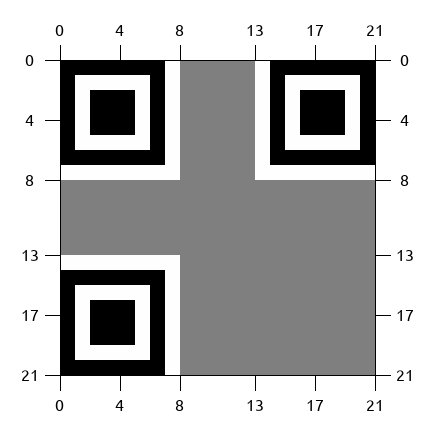
\includegraphics[width=0.4\textwidth]{images/qr_sep_finder}
  \caption{QR-Code example: separators and finder patterns}
  \label{fig:qr_sep_finder}
\end{figure}

\subsection{Alignment patterns}
\label{ssec:qr_alignment}

The next element to add are the alignment patterns. These are similar to finder patterns but are only 5x5. They are spread across the whole code and provide reference points for the scannnig device to improve reliability. The larger the code, the more alignment patterns are needed. Their positions depend on the version and are referenced in table \ref{tab:qr_alignment}. This table lists all possible x and y coordinates for the patterns. This means that for version 2, the alignment patterns are located at (6,6), (6,18), (18,6) and (18,18). A pattern will only be present if the area it covers is still empty (i.e. it doesn't overlap with the separators and finder patterns).

Since our example is a version 1 QR-Code, no alignment pattern is needed (see figure \ref{fig:qr_reserved} for version 10 code with alignment patterns).

\subsection{Timing pattern}
\label{ssec:qr_timing}

An additional element helping the scanner and improving readability is the timing pattern. It consists of a alternating black and white stripe joining the bottom-left and top-left finder pattern, and the top-left and top-right.

The pattern is aligned to the right and bottom borders of the top-left finder patterns, starting with white on the separators.

\begin{figure}[H]
  \centering
  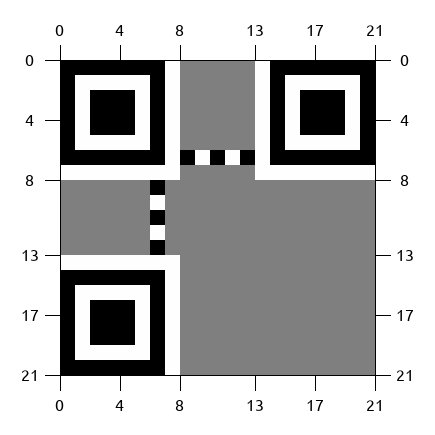
\includegraphics[width=0.4\textwidth]{images/qr_timing}
  \caption{QR-Code example: timing patterns}
  \label{fig:qr_timing}
\end{figure}

\subsection{Reserved area}
\label{ssec:qr_reserved}

Some areas of the matrix are also reserved for format information which will be added later. This corresponds to the modules around the top-left finder pattern, the modules on the right of the bottom-left pattern and those just below the top-right one.

Additionally, for versions greater than 6, a 3x6 zone on the left of the top-right finder pattern plus a 6x3 above the bottom-left one are reserved for version information.

Figure \ref{fig:qr_reserved} shows an example of these reserved areas (in light gray) for a version 10 QR-Code (left) and for our example (right).

\begin{figure}[H]
  \centering
  \raisebox{-0.5\height}{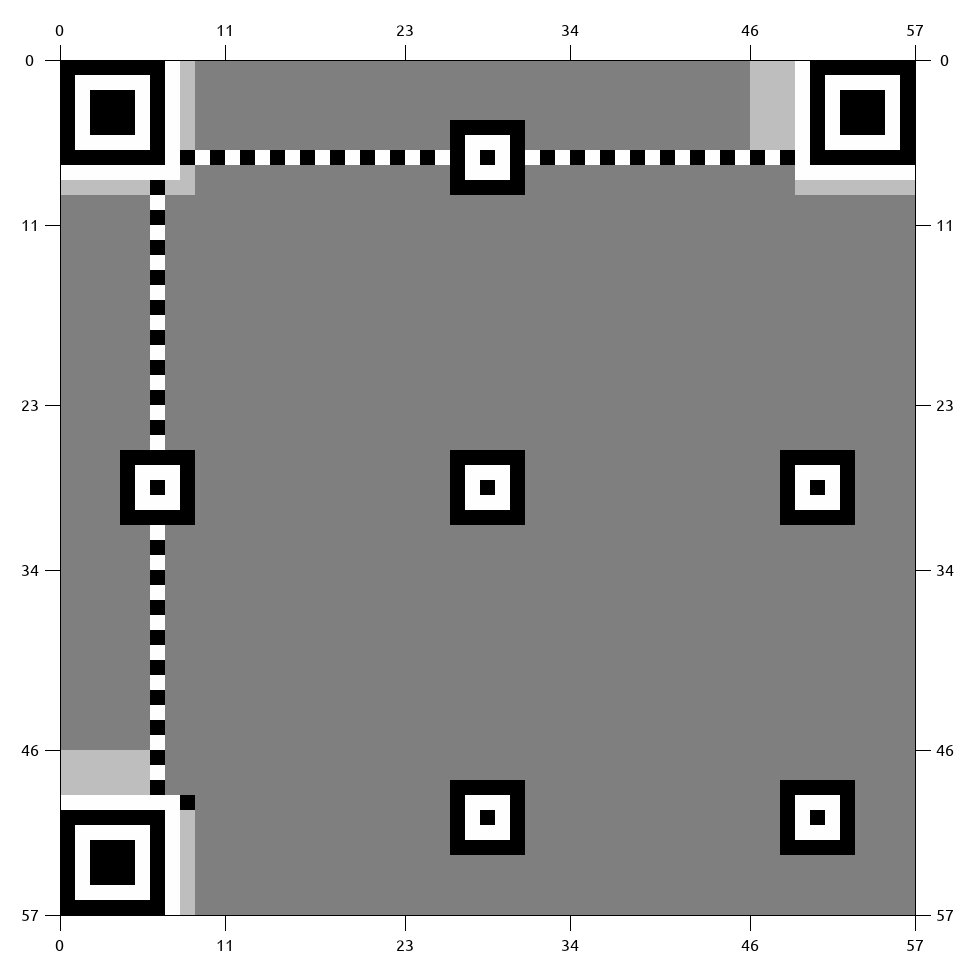
\includegraphics[width=0.5\textwidth]{images/qr_reserved_example}}
  \raisebox{-0.5\height}{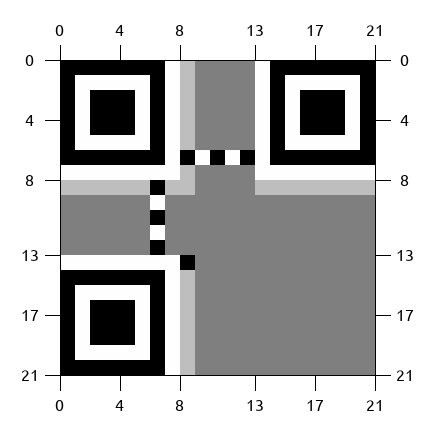
\includegraphics[width=0.4\textwidth]{images/qr_reserved}}
  \caption{QR-Code example: reserved areas}
  \label{fig:qr_reserved}
\end{figure}

A black module is also set next to the bottom-left finder pattern, on the right of its top-right corner. Its coordinates are the following:
\begin{math}
  \begin{cases}
    x = 8 \\
    y = 4V + 9
  \end{cases}
\end{math}
where $V$ is the version.

\subsection{Data placement}
\label{ssec:qr_placement}

The matrix is now ready to receive the data bit string. The placement is done in zigzags, starting from the bottom-right, going up. Each byte is placed in a 2 modules wide region in a staggered manner. When a pattern, separator or reserved area is encountered, the position is skipped and the process continues further.

Figures \ref{fig:qr_plcmt_byte_up} and \ref{fig:qr_plcmt_byte_down} represent the way a byte is layed out when going up or down.

Figures \ref{fig:qr_plcmt_reserved} and \ref{fig:qr_plcmt_turning} show how skipping and turning are processed.

When encountering the vertical timing pattern, that column is entirely skipped and the placement continues on the next one. For each byte, the bits are layed from Most Significant bit (MSB) to Least Significant Bit (LSB).

\begin{figure}[H]
  \centering
  \begin{subfigure}{0.3\textwidth}
    \centering
    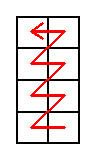
\includegraphics[width=0.5\textwidth]{images/qr_plcmt_byte_up}
    \caption{Going up}
    \label{fig:qr_plcmt_byte_up}
  \end{subfigure}
  \begin{subfigure}{0.3\textwidth}
    \centering
    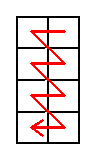
\includegraphics[width=0.5\textwidth]{images/qr_plcmt_byte_down}
    \caption{Going down}
    \label{fig:qr_plcmt_byte_down}
  \end{subfigure}
  \begin{subfigure}{0.3\textwidth}
    \centering
    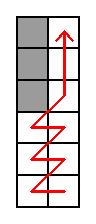
\includegraphics[width=0.5\textwidth]{images/qr_plcmt_reserved}
    \caption{Skipping reserved areas}
    \label{fig:qr_plcmt_reserved}
  \end{subfigure}
  \begin{subfigure}{0.3\textwidth}
    \centering
    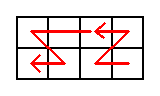
\includegraphics[width=0.7\textwidth]{images/qr_plcmt_turning}
    \caption{Turning at border}
    \label{fig:qr_plcmt_turning}
  \end{subfigure}
  \caption{QR-Code byte placement}
  \label{fig:qr_plcmt_byte}
\end{figure}

\begin{comment}
\begin{figure}[H]
  \centering
  \begin{subfigure}{0.3\textwidth}
    \centering
    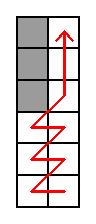
\includegraphics[width=0.3\textwidth]{images/qr_plcmt_reserved}
    \caption{Skipping reserved areas}
    \label{fig:qr_plcmt_reserved}
  \end{subfigure}
  \begin{subfigure}{0.6\textwidth}
    \centering
    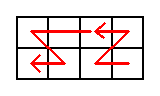
\includegraphics[width=0.5\textwidth]{images/qr_plcmt_turning}
    \caption{Turning at border}
    \label{fig:qr_plcmt_turning}
  \end{subfigure}
  \caption{QR-Code byte placement}
  \label{fig:qr_plcmt_byte_special}
\end{figure}
\end{comment}

If the available space if not fully filled after placing the data, the rest is filled with 0s\footnote{it shall be recalled that 0 means white and 1 means black}.

Our example QR-Code, once filled with data, looks like this:

\begin{figure}[H]
  \centering
  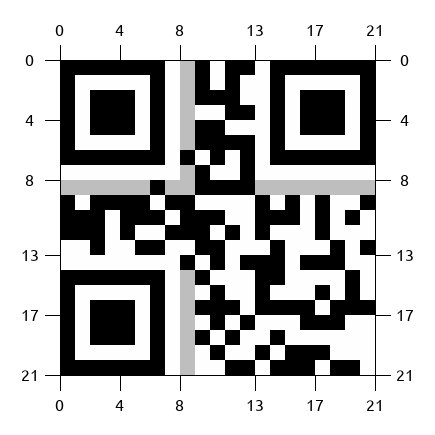
\includegraphics[width=0.4\textwidth]{images/qr_plcmt}
  \caption{QR-Code example: data placement}
  \label{fig:qr_plcmt}
\end{figure}

\subsection{Masking}
\label{ssec:qr_masking}

For optimal readability, it is important that certain patterns of modules don't appear inside the code. For example, there shouldn't be any shape resembling the finder or alignment patterns (i.e. modules with the ratio 1:1:3:1:1). Furthermore, a balanced amount of black compared to white is preferred for better decoding.

For this purpose, we need to apply a mask on the code, switching white for black modules and vice versa where it applies. QR-Codes have 8 different masks which can be used. Obviously, these are only applicable on the data area and should not modify the timing, finder and alignment patterns.

To choose one, we will apply them one after the other on our current QR-Code, and evaluate the resulting code, giving it a penalty score for each undesired feature. Then, the mask with the lowest score will be chosen.

Figure \ref{fig:qr_masks} lists the different possible masks.
A black mask module means that the corresponding data module needs to be inverted.
The operator "//" is integer division.

\begin{figure}[H]
  \centering
  \begin{subfigure}{0.4\textwidth}
    \centering
    
\includegraphics[width=0.4\textwidth]{images/qr_mask_0}
    \caption{(x+y) mod 2 = 0}
    \label{fig:qr_mask_0}
  \end{subfigure}
  \begin{subfigure}{0.4\textwidth}
    \centering
    
\includegraphics[width=0.4\textwidth]{images/qr_mask_1}
    \caption{y mod 2 = 0}
    \label{fig:qr_mask_1}
  \end{subfigure}
  \begin{subfigure}{0.4\textwidth}
    \centering
    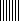
\includegraphics[width=0.4\textwidth]{images/qr_mask_2}
    \caption{(x) mod 3 = 0}
    \label{fig:qr_mask_2}
  \end{subfigure}
  \begin{subfigure}{0.4\textwidth}
    \centering
    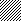
\includegraphics[width=0.4\textwidth]{images/qr_mask_3}
    \caption{(x+y) mod 3 = 0}
    \label{fig:qr_mask_3}
  \end{subfigure}
  \begin{subfigure}{0.4\textwidth}
    \centering
    
\includegraphics[width=0.4\textwidth]{images/qr_mask_4}
    \caption{(y//2+x//3) mod 2 = 0}
    \label{fig:qr_mask_4}
  \end{subfigure}
  \begin{subfigure}{0.4\textwidth}
    \centering
    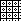
\includegraphics[width=0.4\textwidth]{images/qr_mask_5}
    \caption{((x*y) mod 2 + (x*y) mod 3) = 0}
    \label{fig:qr_mask_5}
  \end{subfigure}
  \begin{subfigure}{0.4\textwidth}
    \centering
    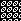
\includegraphics[width=0.4\textwidth]{images/qr_mask_6}
    \caption{((x*y) mod 2 + (x*y) mod 3) mod 2 = 0}
    \label{fig:qr_mask_6}
  \end{subfigure}
  \begin{subfigure}{0.4\textwidth}
    \centering
    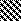
\includegraphics[width=0.4\textwidth]{images/qr_mask_7}
    \caption{((x+y) mod 2 + (x*y) mod 3) mod 2 = 0}
    \label{fig:qr_mask_7}
  \end{subfigure}
  \caption{QR-Code masks}
  \label{fig:qr_masks}
\end{figure}


\subsubsection{Evaluation}
\label{sssec:qr_mask_eval}

Evaluation of a mask is done thanks to 4 criteria.

They evaluate whether the code is easy to read or not. For example, criterion 3 gives a high penalty for every pattern with the same proportions as finder patterns to avoid confusion for the reading device.

Before applying a mask for evaluation, format and version information have do be added on the code, as described in sections \ref{ssec:qr_fmt_info} and \ref{ssec:qr_ver_info}.

\begin{enumerate}
  \item 5+ consecutive modules of the same color:

  If a line or column of 5 or more modules of the same color is found in the code, a penalty score is added. For a strip of $5 + i$ same colored modules, the penalty is worth $3 + i$ points.

  \item 2x2 blocks:

  Each 2x2 block of similar modules adds 3 points to the penalty score. Overlapping blocks are taken into account.

  \item 1:1:3:1:1:4 patterns:

  For each pattern with the ratios 1:1:3:1:1:4 or 4:1:1:3:1:1, a penalty of 40 points is given. This criterion takes into account the 4-module wide margins all around the code\footnote{see \autoref{ssec:qr_sep_finder}}. This means there are at least 18 correspondances in every code.

  \item Proportion of black and white modules:

  A penalty is attributed according to the deviation from a 50/50 distribution in black and white modules across the whole QR-Code. The calculation method is the following:
  \[ P = \lfloor 100 * B / (W*H) \rfloor \]
  \[ P_1 = P - P \textrm{ mod } 5 \]
  \[ P_2 = P_1 + 5 \]
  \[ S = \textrm{min}\left(\frac{|P_1 - 50|}{5}, \frac{|P_2 - 50|}{5}\right) * 10 \]
\end{enumerate}

where $B$ is the total number of black modules, $W$ and $H$ are the width and height of the QR-Code, and $S$ is the penalty score given for this criterion.

Applying this to our QR-Code, we can determine that the best mask is mask \ref{fig:qr_mask_5} with a score of 442. Figures \ref{fig:qr_mask_ex_eval_1} to \ref{fig:qr_mask_ex_eval_4} detail the penalties for each criterion.

\begin{figure}[H]
  \centering
  \begin{subfigure}{0.45\textwidth}
    \centering
    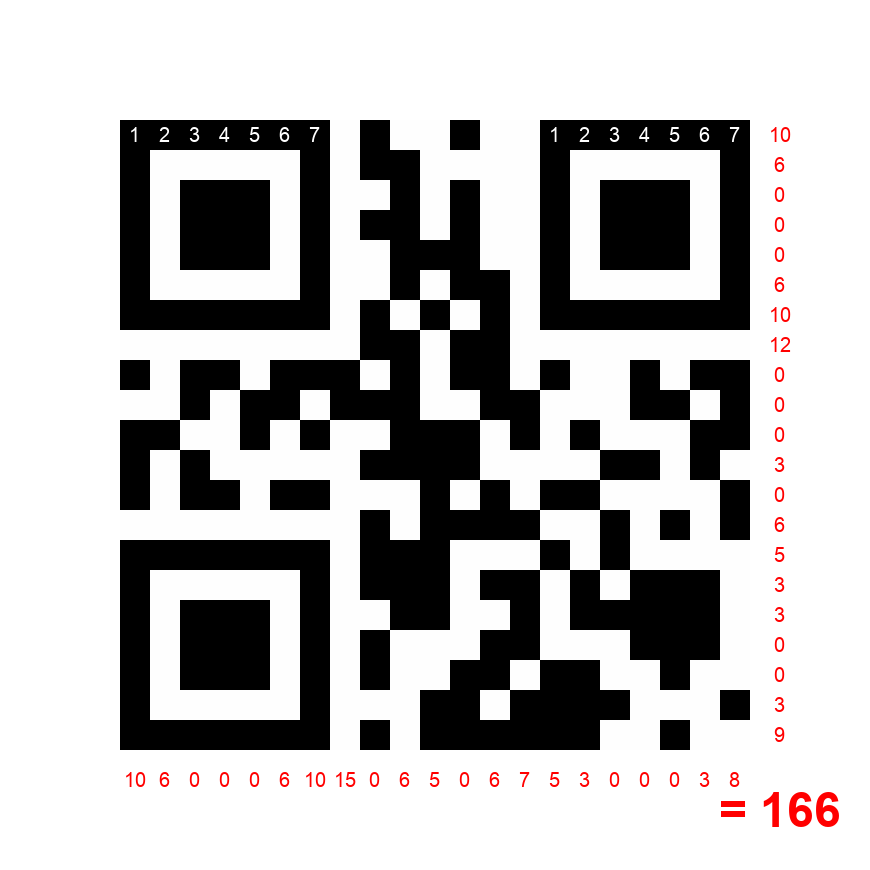
\includegraphics[width=\textwidth]{images/qr_mask_ex_eval_1}
    \caption{QR-Code example: mask evaluation (1)}
    \label{fig:qr_mask_ex_eval_1}
  \end{subfigure}
  \begin{subfigure}{0.45\textwidth}
    \centering
    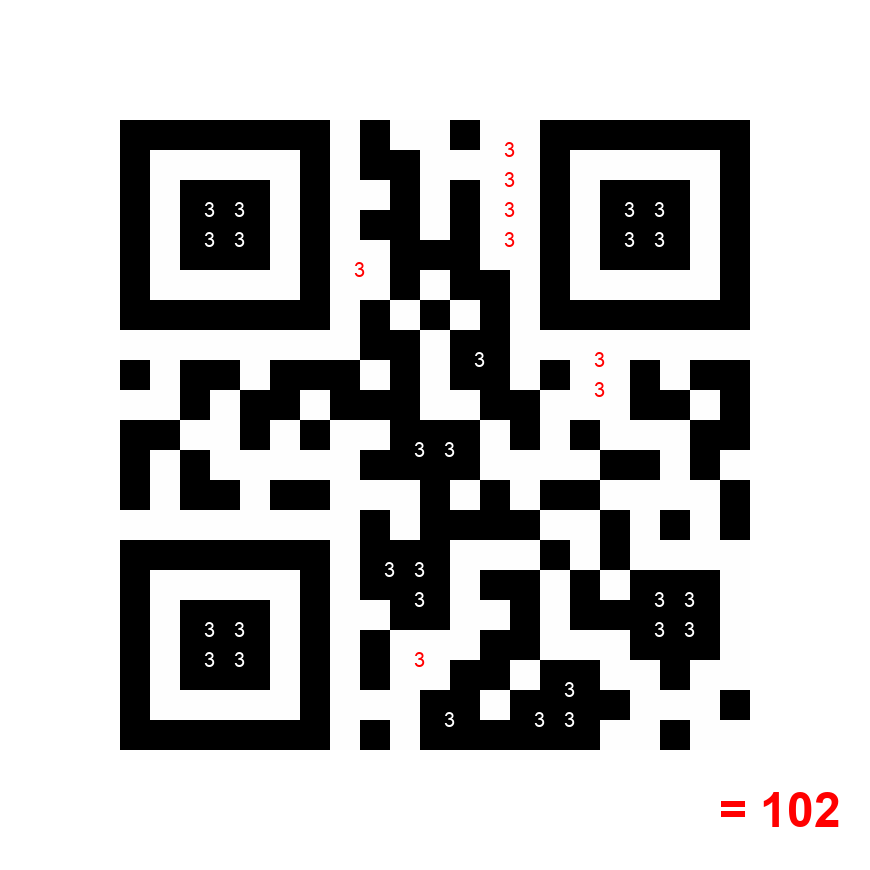
\includegraphics[width=\textwidth]{images/qr_mask_ex_eval_2}
    \caption{QR-Code example: mask evaluation (2)}
    \label{fig:qr_mask_ex_eval_2}
  \end{subfigure}
  \begin{subfigure}{0.45\textwidth}
    \centering
    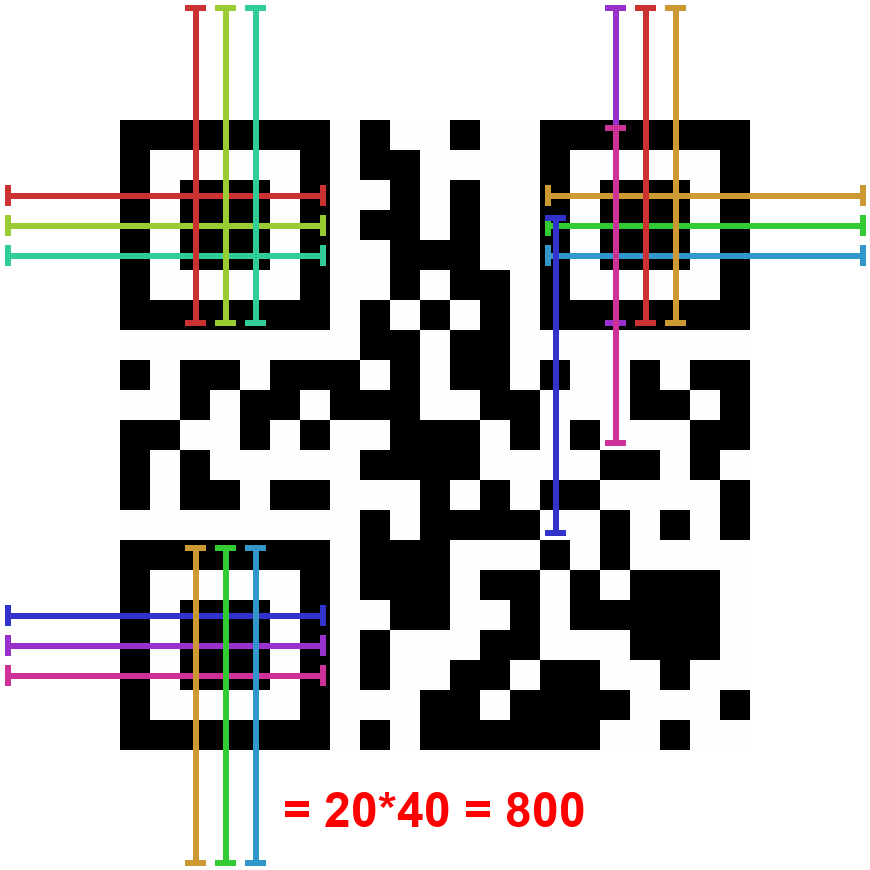
\includegraphics[width=\textwidth]{images/qr_mask_ex_eval_3}
    \caption{QR-Code example: mask evaluation (3)}
    \label{fig:qr_mask_ex_eval_3}
  \end{subfigure}
  \begin{subfigure}{0.45\textwidth}
    \centering
    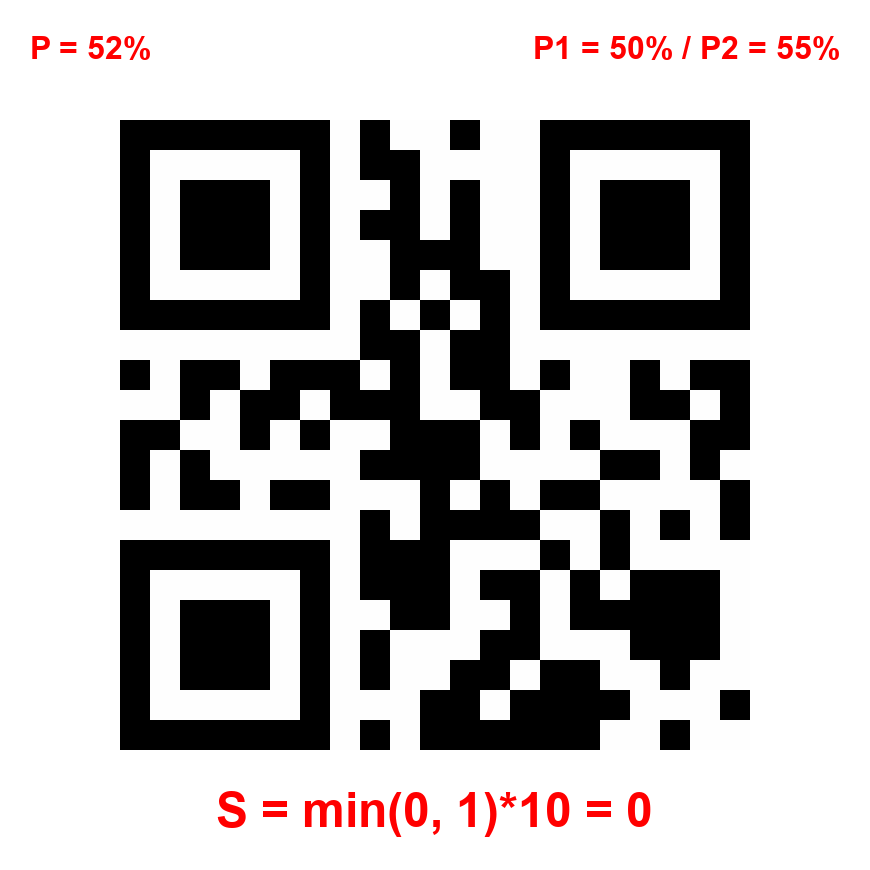
\includegraphics[width=\textwidth]{images/qr_mask_ex_eval_4}
    \caption{QR-Code example: mask evaluation (4)}
    \label{fig:qr_mask_ex_eval_4}
  \end{subfigure}
  \caption{QR-Code example: mask evaluation}
  \label{fig:qr_mask_ex_eval}
\end{figure}

\subsection{Format information}
\label{ssec:qr_fmt_info}

The last step to complete a fully functional QR-Code is to add the format information, and version information for versions bigger than 6.

First we need to create a format string containing the level of error correction and the mask used. The correction level is encoded on 2 bits as follows:

\begin{table}[H]
  \centering
  \begin{tabu}{|c|c|}
    \hline
    Level & Value (bin) \\
    \hline
    L & 01 \\
    \hline
    M & 00 \\
    \hline
    Q & 11 \\
    \hline
    H & 10 \\
    \hline
  \end{tabu}
  \caption{QR-Code error correction level indicator}
  \label{tab:qr_ec_ind}
\end{table}

Then the mask id is converted to a 3-bit binary number and appended to the error correction level indicator.

The string is padded by an additional 10 0s to make it 15 bits long.

Similarly to what has been done with data previously, the format string is complemented with error correction bits, this time using Bose-Chaudhuri-Hocquenghem (BCH) codes.
The principle is similar to the Reed-Solomon algorithm in that a message polynomial is divided by a generator polynomial. To create the message polynomial, each bit of the format string represents the coefficient of a term. The same applies for the generator polynomial, which is always derived from the binary number \texttt{10100110111}.
The generator polynomial is thus \[
  x^{10} + x^8 + x^5 + x^4 + x^2 + x + 1
\]

The division's remainder is then padded on the left with 0s to make it 10 bits long.

The final bit string is constructed by concatenating the format string with the error correction bits, and XORing\footnote{With the binary XOR operator} the result with the mask string \texttt{101010000010010}. This mask ensures the final format string is not made of only 0s.

Once calculated, the bit string is layed out in the reserved strips around the finder patterns, as shown in figure \ref{fig:qr_fmt_layout} (0 being the LSB and 14 the MSB)

\begin{figure}[H]
  \centering
  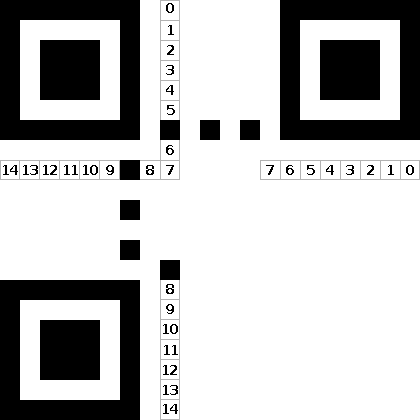
\includegraphics[width=0.4\textwidth]{images/qr_fmt_layout}
  \caption{QR-Code format information string layout}
  \label{fig:qr_fmt_layout}
\end{figure}

It is to be noted that format information appears twice, since its decoding is essential for reading the whole code.

In our case, the error correction indicator for level M is 00 and we used the mask with id 2, so our format string is \texttt{000100000000000}. Dividing it by the generator polynomial yields the remainder \texttt{1001101110}.

Adding it to the format string and XORing it with the mask string, we get \texttt{101111001111100}.

These bits are then put in the reserved areas of the matrix, making figure \ref{fig:qr_fmt_info}

\begin{figure}[H]
  \centering
  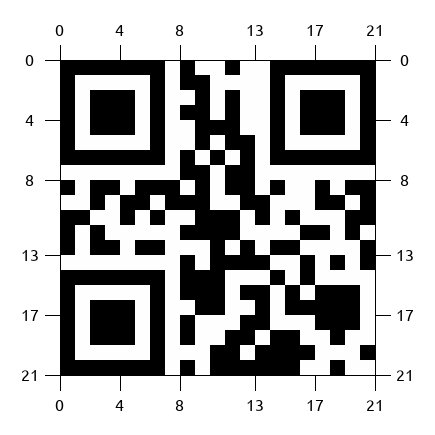
\includegraphics[width=0.4\textwidth]{images/qr_fmt_info}
  \caption{QR-Code example: format information}
  \label{fig:qr_fmt_info}
\end{figure}

Our QR-Code is now fully finished and can be scanned.

\subsection{Version information}
\label{ssec:qr_ver_info}

For QR-Codes of version 7 and bigger, additional data is added to state the code's version.

To generate the version string, first convert the version to its 6 bit binary representation. Then append the remainder of the division by the generator polynomial \[
  x^{12} + x^{11} + x^{10} + x^9 + x^8 + x^5 + x^2 + 1
\] padded on the left to 12 bits, following the same methods as for format information.

This string is then put in the two reserved 6x3 and 3x6 rectangles. The LSB is placed in the top-left corner of the rectangles. For the top-right area, the string goes down, then to the right. For the bottom-left rectangle, the string goes to the right, then down.
